\documentclass[12pt]{article}

\usepackage[utf8]{inputenc}
\usepackage{latexsym,amsfonts,amssymb,amsthm,amsmath}
\usepackage{float}

\setlength{\parindent}{0in}
\setlength{\oddsidemargin}{0in}
\setlength{\textwidth}{6.5in}
\setlength{\textheight}{8.8in}
\setlength{\topmargin}{0in}
\setlength{\headheight}{18pt}
\usepackage{graphicx}

\usepackage{caption}
\DeclareCaptionFormat{citation}{%
  \ifx\captioncitation\relax\relax\else
    \captioncitation\par
  \fi
  #1#2#3\par}
\newcommand*\setcaptioncitation[1]{\def\captioncitation{\textit{Source:}~#1}}
\let\captioncitation\relax
\captionsetup{format=citation,justification=centering}


\title{MATH1034OL1 Pre-Calculus Mathematics Notes from Sections 4.5, 1.6, 2.3 (Monday)}
\author{Elijah Renner}

\begin{document}

\maketitle

\vspace{0.5in}

\tableofcontents


\section{Review Problems}


\subsection{\(\text{Problem: Evaluate }
\cot \left( \frac{2\pi}{3} \right)\)}

First, we determine the reference angle. Since \(\frac{2\pi}{3}=\frac{2\pi}{3}\cdot\frac{180^{\circ}}{\pi}=120^{\circ}\), the angle is in the second quadrant. Recall from July 5th's notes that to find the reference angle of an angle in the second quadrant, we subtract it from \(180^{\circ}\) or \(\pi\). Since we're working toward being comfortable with radian measures, we'll perform this operation in radians:\\

\[\text{reference angle}=\pi-\frac{2\pi}{3}=\frac{3\pi}{3}-\frac{2\pi}{3}=\frac{\pi}{3}\]

This tells us we're dealing with a 30-60-90 triangle. Now, let's recall that \(\cot=\frac{\text{adj}}{\text{opp}}\). Let's look for those.

\begin{figure}[H]
	\centering
	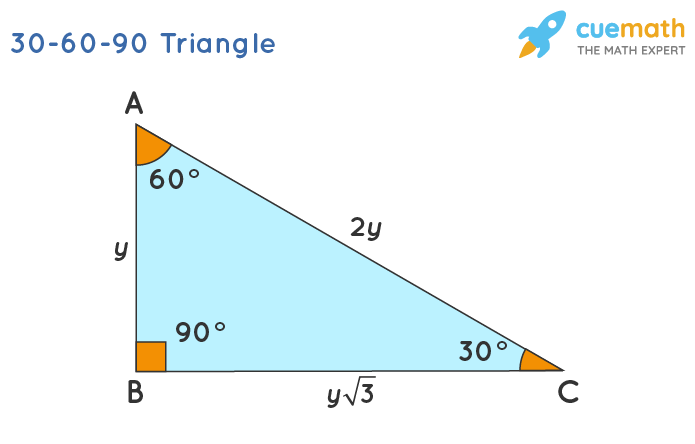
\includegraphics[scale=0.5]{30-60-90-triangle-1621153010.png}
	\caption{Credit: https://www.cuemath.com/geometry/30-60-90-triangle/}
\end{figure}

Here, \(y=\frac{1}{2}\). So, \(\text{opp}=\frac{\sqrt{3}}{2}\) and \(\text{adj}=\frac{1}{2}\). Thus, \(\cot\left( \frac{2\pi}{3}\right) =\frac{\text{adj}}{\text{opp}}=\frac{\frac{1}{2}}{\frac{\sqrt{3}}{2}}=\frac{1}{2}\cdot\frac{2}{\sqrt{3}}=\frac{1}{\sqrt{3}}\cdot\frac{\sqrt{3}}{\sqrt{3}}=\frac{\sqrt{3}}{3}\)\\

Don't forget that \(\cot\left( \frac{2\pi}{3}\right)=-\frac{\sqrt{3}}{3}\) because \(\cot\) is negative in quadrant two.

\subsection{\(\text{Graph } y=2\sin(4x-20^{\circ})-3\)}


When graphing sinosodal functions, we must determine amplitude, period, sub-period, phase (horizontal) shift, vertical shift, and shape:\\

\begin{figure}[H]
	\centering
	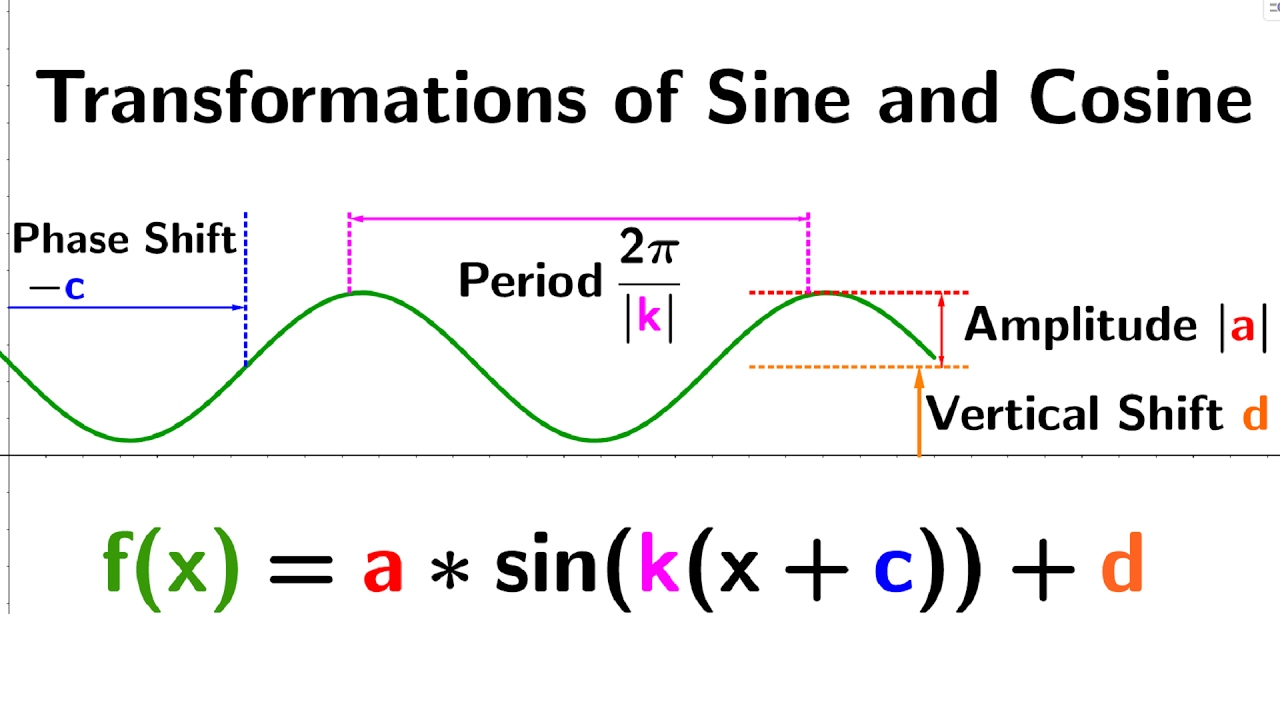
\includegraphics[scale=0.2]{maxresdefault.jpg}
	\caption{Credit: https://youtu.be/AS7THLj-OhI}
\end{figure}

We first factor the \(4x-20^{\circ}\): \(y=2\sin(4x-20^{\circ})-3=2\sin(4(x-5^{\circ}))-3\).

Now, \(a=2, k=4, c=-5, \text{and } d=-3\).\\

Thus, amplitude = \(|a|=|2|=2\), period = \(\frac{2\pi}{|k|}=\frac{2\pi}{4}=\frac{\pi}{2}\), sub-period = \(\frac{\text{period}}{4}=\frac{\pi}{8}\), phase shift = \(-c=5\), vertical shift = \(d=-3\).\\

Since \(a>0\), the graph opens up. With these properties, the function can be graphed.\\

\section{Trigonometric Functions on the Unit Circle}

On the unit circle with angle \(\theta\), \(x=\cos\theta\) and \(y=\sin\theta\):\\

\begin{figure}[H]
	\centering
	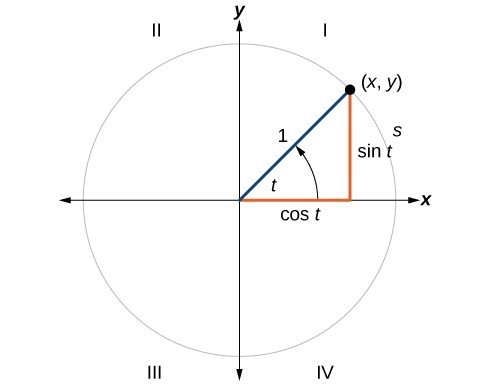
\includegraphics[scale=0.5]{CNX_Precalc_Figure_05_02_0022.jpg}
	\caption{Credit: https://courses.lumenlearning.com/precalculus/chapter/unit-circle-sine-and-cosine-functions/}
\end{figure}

Hence, \\

\begin{align*}
\tan\theta &= \frac{y}{x} = \frac{\sin\theta}{\cos\theta} \quad (x \neq 0) \\
\csc\theta &= \frac{1}{y} \quad (y \neq 0) \\
\sec\theta &= \frac{1}{x} \quad (x \neq 0) \\
\cot\theta &= \frac{x}{y} =  \frac{\cos\theta}{\sin\theta} \quad (y \neq 0) \\
\end{align*}

\section{Domain and Range}

Polynomials all have domain \(\mathbb{R}\).\\

For even degree polynomials, the range is restricted.\\

For odd degree polynomials, the range is \(\mathbb{R}\).\\

Rational functions have a domain of \(\mathbb{R}\) excluding the values that make the denominator equal to zero. Example:\\

for \(g(x)=\frac{x-2}{5x+15}\), \(5x+15 \neq 0 \).\\

\(\implies 5x\neq-15\)\\

\(\implies x \neq -3\)\\

Hence, the domain of \(g\) can be written as \(\{ x \in \mathbb{R} \mid x\neq-3\}\).\\

Even root functions, such as \(h(x)=\sqrt{4x+1}\), have domains of all values \(x\) such that the contents of the root aren't negative. For \(h\), \(4x+1\geq0.\)\\

\(\implies 4x\geq-1\)\\

\(\implies x\geq-\frac{1}{4}\)\\

So the domain of \(h\) is \([-\frac{1}{4},\infty)\).\\

Conversely, odd root functions have domains \(\mathbb{R}\).

\section{Limit Definition of the Derivative}
The derivative of a function \( f(x) \) at a point \( x = a \) is defined by the limit:

\[
f'(a) = \lim_{{h \to 0}} \frac{f(a+h) - f(a)}{h}
\]

Let's apply this definition to the function \( f(x) = x^2 - x + 2 \).

First, we need to compute \( f(a+h) \):

\[
f(a+h) = (a+h)^2 - (a+h) + 2
\]

Expanding this, we get:

\[
f(a+h) = a^2 + 2ah + h^2 - a - h + 2
\]

Next, we compute \( f(a) \):

\[
f(a) = a^2 - a + 2
\]

Now, we find the difference \( f(a+h) - f(a) \):

\[
f(a+h) - f(a) = (a^2 + 2ah + h^2 - a - h + 2) - (a^2 - a + 2)
\]

Simplifying, we get:

\[
f(a+h) - f(a) = 2ah + h^2 - h
\]

We then divide by \( h \):

\[
\frac{f(a+h) - f(a)}{h} = \frac{2ah + h^2 - h}{h} = 2a + h - 1
\]

Finally, we take the limit as \( h \) approaches 0:

\[
f'(a) = \lim_{{h \to 0}} (2a + h - 1) = 2a - 1
\]

Therefore, the derivative of the function \( f(x) = x^2 - x + 2 \) is:

\[
f'(x) = 2x - 1
\]

To find the slope of the function at \( x = 5 \), we substitute \( x = 5 \) into the derivative:

\[
f'(5) = 2(5) - 1
\]

Simplifying, we get:

\[
f'(5) = 10 - 1 = 9
\]

Therefore, the slope of the function \( f(x) = x^2 - x + 2 \) at the point \( x = 5 \) is:

\[
f'(5) = 9
\]

Now, let's use the point-slope form to find the equation of the tangent line at \( x = 5 \).

The point-slope form of the equation of a line is given by:

\[
y - y_1 = m(x - x_1)
\]

where \( m \) is the slope of the line and \((x_1, y_1)\) is a point on the line.

In our case, the slope \( m \) is \( 9 \), and the point \((x_1, y_1)\) is \((5, f(5))\).

First, we need to find \( f(5) \):

\[
f(5) = 5^2 - 5 + 2 = 25 - 5 + 2 = 22
\]

So the point is \((5, 22)\).

Now, we can substitute \( m = 9 \), \( x_1 = 5 \), and \( y_1 = 22 \) into the point-slope form:

\[
y - 22 = 9(x - 5)
\]

Simplifying, we get:

\[
y - 22 = 9x - 45
\]

\[
y = 9x - 45 + 22
\]

\[
y = 9x - 23
\]

Therefore, the equation of the tangent line to the function \( f(x) = x^2 - x + 2 \) at the point \( x = 5 \) is:

\[
y = 9x - 23
\]


\end{document}
